\documentclass[../DoAn.tex]{subfiles}
\begin{document}

Chương này trình bày các cơ sở lý thuyết mà đồ án dựa vào: đặc điểm
các nhóm mã độc trên Windows, định dạng tệp PE và đặc trưng tĩnh, các
thuật toán học máy dùng để phân loại, cơ chế giám sát hành vi động bằng
Sysmon và ETW, cùng khung MITRE ATT\&CK; phần cuối điểm qua các công
trình liên quan.

\section{Phần mềm độc hại}
\label{section:2.1}

Phần mềm độc hại là các chương trình được thiết kế nhằm xâm nhập, 
gây hại hoặc khai thác trái phép hệ thống máy tính mà không có sự 
đồng ý của người dùng~\cite{ye2017}. Tùy theo cơ chế hoạt động và 
mục tiêu tấn công, phần mềm độc hại được phân loại thành nhiều nhóm~\cite{gibert2020}. Bảng~\ref{tab:malware_comparison} tổng hợp đặc điểm, cách lan truyền
và hành vi quan sát được trong sandbox của bảy nhóm được đánh giá
trong đồ án.
\begin{table}[H]
\centering
\caption{So sánh các nhóm phần mềm độc hại và hành vi quan sát được
  trong sandbox, tổng hợp từ các
  nguồn~\cite{ye2017,gibert2020,DBLP:journals/corr/abs-2102-06249,7958609,rezaeirad2018,rashid2024,Zou2006,porras2009}.}
\label{tab:malware_comparison}
\begin{tabular}{|l|p{3cm}|p{2.6cm}|p{5.5cm}|}
\hline
\multicolumn{1}{|c|}{\textbf{Nhóm}} & \multicolumn{1}{c|}{\textbf{Đặc điểm chính}} & \multicolumn{1}{c|}{\textbf{Lan truyền}} & \multicolumn{1}{c|}{\textbf{Hành vi đặc trưng trong sandbox}} \\
\hline
Dropper & Tải và cài payload thứ cấp & Qua người dùng & Giải nén hoặc tải tệp thực thi mới, tạo tiến trình con, thiết lập tự khởi động \\
\hline
Ransomware & Mã hóa dữ liệu, đòi tiền chuộc & Qua người dùng & Đọc/ghi/đổi tên hàng loạt tệp, xóa Shadow Copy, dừng dịch vụ bảo mật, kết nối C2 \\
\hline
Trojan & Ngụy trang phần mềm hợp lệ & Qua người dùng & Tạo tiến trình con bất thường, ghi tệp thực thi mới, thiết lập tự khởi động, kết nối C2 \\
\hline
RAT & Điều khiển từ xa hai chiều & Qua người dùng & Kết nối TCP từ tiến trình không phải trình duyệt, beacon định kỳ, ghi bàn phím, chụp màn hình, nạp assembly .NET trong bộ nhớ \\
\hline
Worm & Tự nhân bản qua mạng & Tự động & Quét TCP/UDP tốc độ cao, tạo bản sao tiến trình, thêm Registry/Service sau thực thi \\
\hline
Cryptominer & Chiếm tài nguyên đào tiền mã hóa & Qua người dùng & Kết nối mining pool, sinh tiến trình đào tiêu thụ CPU cao, thiết lập tự khởi động \\
\hline
Spyware & Thu thập thông tin bí mật & Qua người dùng & Ghi bàn phím, đọc tệp và dữ liệu trình duyệt, gửi dữ liệu thu thập ra C2 \\
\hline
\end{tabular}
\end{table}
\section{Định dạng tệp PE và đặc trưng tĩnh}
\label{section:2.2}

PE là định dạng tệp thực thi chủ đạo
trên hệ điều hành Microsoft Windows, bao gồm các tệp thực
thi (\texttt{.exe}) và thư viện liên kết động
(\texttt{.dll}).
Vì hầu hết phần mềm độc hại trên Windows đều tồn tại dưới
dạng tệp PE, phân tích tĩnh cấu trúc PE mà không cần thực
thi tệp trở thành một lớp bảo vệ quan trọng trong hệ thống
phát hiện mã độc~\cite{ember2018}.

\subsection{Cấu trúc tệp PE}
\label{section:2.2.1}

\begin{figure}[H]
  \centering
  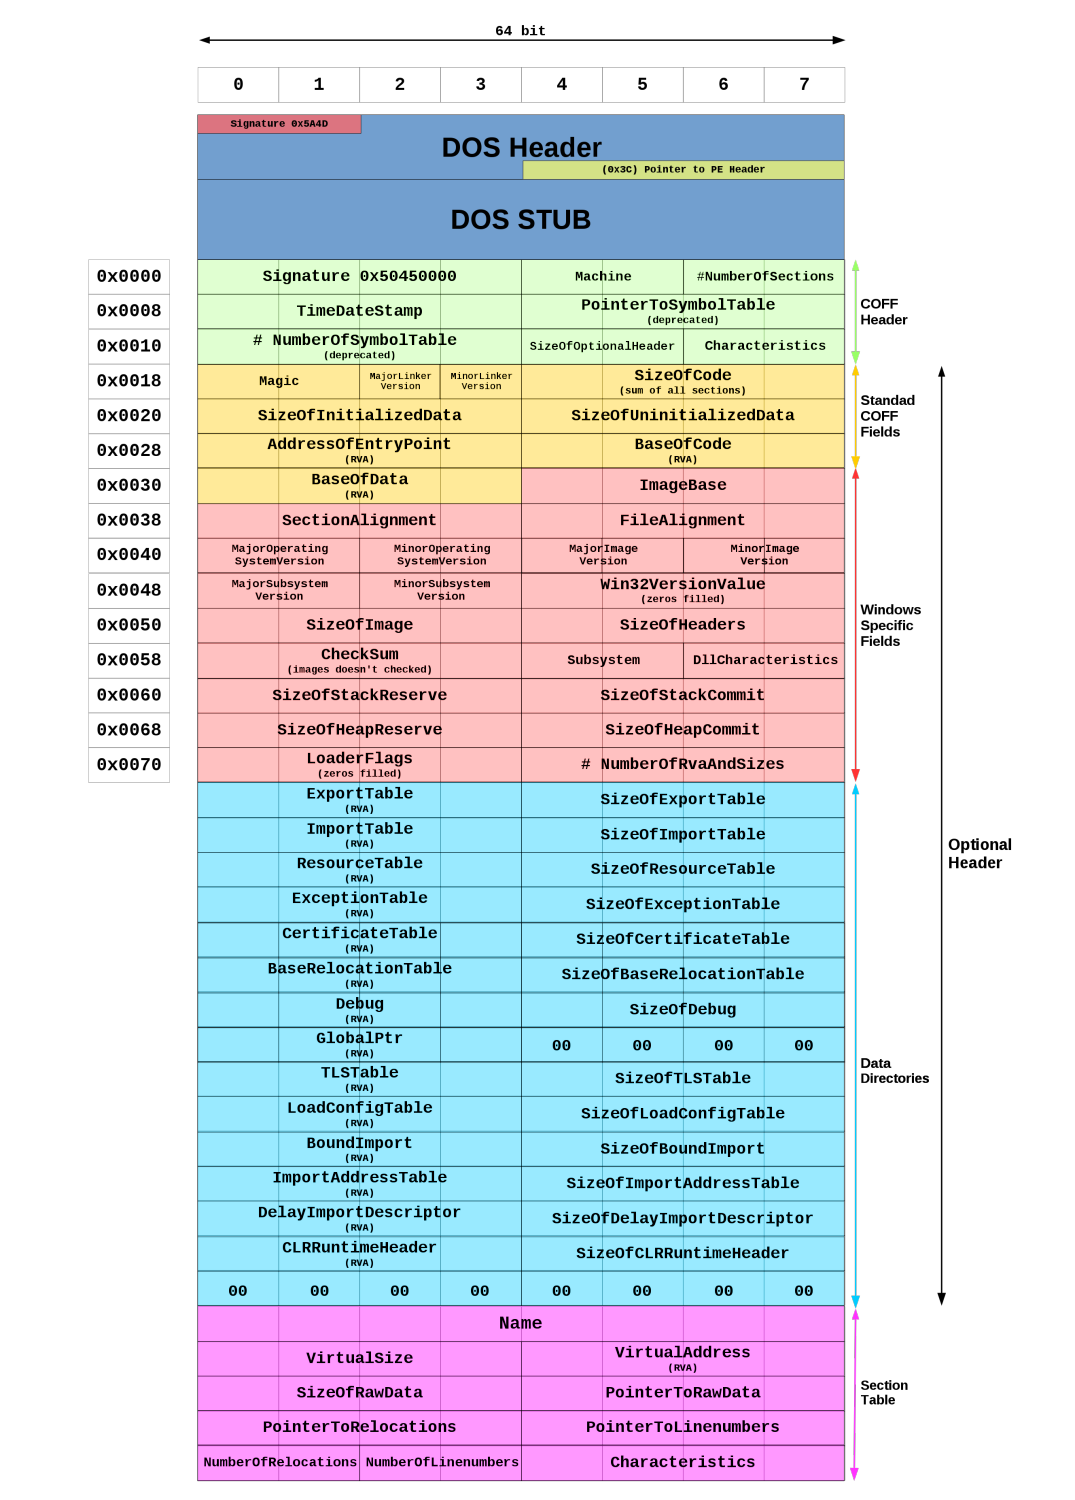
\includegraphics[width=0.9\linewidth]{Hinhve/Pic1_pe_structure.png}
  \caption{Cấu trúc tệp PE 32-bit~\cite{ember2018}.}
  \label{fig:pe_structure}
\end{figure}
Tệp PE được tổ chức thành hai phần chính: phần header và các section,
như minh họa trong Hình~\ref{fig:pe_structure}~\cite{ember2018}. Phần
header bao gồm COFF Header (kiến trúc máy đích, số section), Optional
Header (entry point, kích thước vùng mã, tham chiếu bảng import/export)
và Section Table (vị trí, kích thước và thuộc tính từng section). Phần
sections chứa mã lệnh và dữ liệu; công cụ đóng gói có thể
thêm section mới để lưu dữ liệu nén hoặc mã được bảo vệ, làm thay đổi
cấu trúc PE và gây khó khăn cho phân tích tĩnh~\cite{ember2018}.
\subsection{Đặc trưng tĩnh dùng trong phát hiện mã độc}
\label{section:2.2.2}

Anderson và Roth đề xuất bộ đặc trưng EMBER gồm tám nhóm đặc trưng
tĩnh~\cite{ember2018}; phiên bản cập nhật bổ sung thêm nhóm Data
Directories, nâng tổng số nhóm lên chín. Cấu hình chín nhóm này cũng
được sử dụng trong nghiên cứu của Choudhary et al.~\cite{choudhary2025}.
Bảng~\ref{tab:ember_features} mô tả các nhóm đặc trưng cùng số chiều
tương ứng.
\begin{table}[H]
\centering
\caption{Chín nhóm đặc trưng tĩnh và số chiều tương ứng~\cite{ember2018, choudhary2025}.}
\label{tab:ember_features}
\begin{tabular}{|l|c|p{8cm}|}
\hline
\multicolumn{1}{|c|}{\textbf{Nhóm đặc trưng}} & \multicolumn{1}{c|}{\textbf{Số chiều}} & \multicolumn{1}{c|}{\textbf{Mô tả}} \\
\hline
Thông tin tổng quát & 10 & Kích thước tệp, số hàm import/export, sự hiện diện của debug, tài nguyên, TLS và chữ ký số \\
\hline
Header & 62 & Các trường từ COFF Header và Optional Header: kiến trúc máy đích, subsystem, cờ DLL \\
\hline
Import & 1.280 & Tên thư viện (256 vị trí hash) và tên hàm import (1.024 vị trí hash) \\
\hline
Export & 128 & Tên các hàm được export \\
\hline
Section & 255 & Tên, kích thước, entropy và thuộc tính của từng section \\
\hline
Chuỗi ký tự & 104 & Thống kê chuỗi có thể in được: đường dẫn, URL, khóa Registry, mẫu ký tự \\
\hline
Histogram byte & 256 & Tần suất của 256 giá trị byte trong toàn bộ tệp \\
\hline
Histogram entropy-byte & 256 & Phân bố kết hợp giữa giá trị byte và entropy cục bộ (lưới $16\times16$) \\
\hline
Data Directories & 30 & Kích thước và địa chỉ ảo của 15 bảng dữ liệu trong PE header \\
\hline
\textbf{Tổng} & \textbf{2.381} & \\
\hline
\end{tabular}
\end{table}
Bốn nhóm có danh sách phần tử dài thay đổi giữa các tệp (tên thư viện,
hàm import/export, tên section) được đưa về vector cố định bằng feature
hashing: mỗi phần tử được một hàm băm ánh xạ vào một vị trí cố định
trong mảng, nhờ đó mọi tệp đều cho ra vector cùng số chiều bất kể số
phần tử nhiều hay ít.

Các đặc trưng tĩnh có ưu điểm là trích xuất nhanh và an toàn mà
không cần môi trường thực thi. Tuy nhiên, các đặc trưng tĩnh dễ bị vô hiệu hóa bởi kỹ thuật đóng
gói: mã thực thi được nén hoặc mã hóa, chỉ giải nén tại
thời điểm chạy, khiến cấu trúc PE quan sát được khác biệt hoàn toàn
so với tệp gốc~\cite{gibert2020}. Hạn chế này là lý do nhiều hệ thống
kết hợp phân tích tĩnh với phân tích động để quan sát hành vi thực tế
của mẫu.

\section{Phân tích tĩnh dựa trên học máy}
\label{section:2.3}
 
\subsection{Hướng tiếp cận học máy trong phát hiện mã độc}
\label{section:2.3.1}
Phương pháp nhận diện dựa trên chữ ký không thể phát hiện các mẫu mã
độc chưa từng được ghi nhận. Học máy khắc phục hạn chế này bằng cách
tự động học các mối quan hệ phức tạp giữa đặc trưng của tệp từ dữ liệu
huấn luyện, tổng quát hóa sang các mẫu mới có phân phối đặc trưng
tương tự~\cite{ember2018}.
 
Quy trình phát hiện mã độc bằng học máy gồm ba bước 
chính~\cite{gibert2020} như minh họa trong 
Hình~\ref{fig:process}: trích xuất đặc trưng từ tệp PE thành vector 
số, huấn luyện mô hình trên tập dữ liệu đã gán nhãn malware hoặc 
benign, và sử dụng mô hình đã huấn luyện để phân loại các tệp mới. 
Chất lượng của bước trích xuất đặc trưng ảnh hưởng trực tiếp đến hiệu
năng phân loại, do đó việc lựa chọn bộ đặc trưng phù hợp đóng vai trò
then chốt trong toàn bộ quy trình~\cite{gibert2020}. Bộ đặc trưng
EMBER 2.381 chiều được trích xuất từ cấu trúc tệp PE; thiết kế cụ thể
được trình bày tại Chương~\ref{chapter:Design}.
\begin{figure}[H]
  \centering
  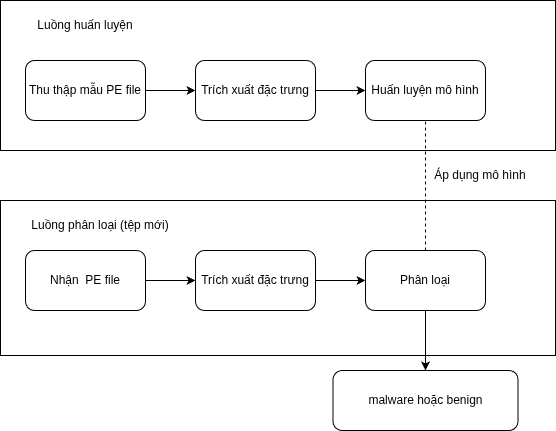
\includegraphics[width=0.8\linewidth]{Hinhve/Pic2Quytrinh.png}
  \caption{Quy trình phát hiện mã độc bằng học máy.}
  \label{fig:process}
\end{figure}
\subsection{Các thuật toán phân loại}
\label{section:2.3.2}

Đồ án đánh giá ba thuật toán phân loại nhị phân trên dữ liệu dạng
bảng: Random Forest, XGBoost và LightGBM.

Random Forest xây dựng nhiều cây quyết định độc lập trên các
tập con dữ liệu và đặc trưng được lấy mẫu ngẫu nhiên, sau
đó tổng hợp kết quả bằng biểu quyết đa số~\cite{breiman2001}. Vì các
cây được xây dựng độc lập với nhau, Random Forest cho phép huấn luyện
song song và chống quá khớp tốt nhờ tính ngẫu nhiên, nhưng không có
cơ chế học từ sai số của cây trước.

XGBoost thuộc họ Gradient Boosting Decision Tree (GBDT), xây
dựng cây tuần tự trong đó mỗi cây học từ sai số của cây
trước~\cite{chen2016xgboost}. So với GBDT truyền thống, XGBoost bổ
sung số hạng phạt vào hàm mục tiêu để giới hạn độ phức tạp của mô
hình và mở rộng cây theo từng tầng, giúp
kiểm soát quá khớp tốt hơn.

LightGBM cũng thuộc họ GBDT nhưng tối ưu hóa tốc độ trên tập
dữ liệu lớn thông qua hai kỹ thuật~\cite{lightgbm2017}: GOSS
ưu tiên giữ lại các mẫu mà mô hình
đang học kém (gradient lớn) và lấy ngẫu nhiên một phần mẫu gradient
nhỏ, giảm số mẫu cần xử lý; EFB gộp các
đặc trưng thưa thớt, giảm số chiều. Khác với XGBoost, LightGBM mở
rộng nút lá có Gain cao nhất, đạt độ chính xác cao hơn
với cùng số vòng học. Kết quả so sánh thực nghiệm được trình bày tại
Chương~\ref{chapter:Experiment}.
\subsection{Lựa chọn đặc trưng dựa trên Importance Gain}
\label{section:2.3.3}
Không phải tất cả đặc trưng đều đóng góp như nhau vào khả năng dự
đoán của mô hình; giữ quá nhiều đặc trưng không chỉ tăng thời gian
huấn luyện mà còn có thể khiến mô hình học nhiễu, làm giảm khả năng
tổng quát hóa~\cite{gibert2020}. Lựa chọn đặc trưng giải quyết vấn
đề này bằng cách chỉ giữ lại những đặc trưng đóng góp cao nhất và
loại bỏ phần còn lại, nhờ đó giảm số chiều mà vẫn duy trì hiệu
năng~\cite{gibert2020}.
 
Với các mô hình dựa trên cây quyết định, cách đánh giá trực tiếp nhất 
là dựa vào chỉ số Importance Gain. Tại mỗi nút trong cây, thuật toán 
chọn đặc trưng giúp tách malware ra khỏi benign rõ nhất; mức độ tách 
này được gọi là Gain. Importance Gain của một đặc trưng là tổng Gain 
mà đặc trưng đó tạo ra trên tất cả các lần được sử dụng để chia, cộng 
dồn qua toàn bộ các cây trong mô hình, như minh họa trong 
Hình~\ref{fig:importance_gain}~\cite{lightgbm2017}. Kết quả là mỗi đặc
trưng nhận một điểm quan trọng duy nhất. Trên thực tế các điểm này rất
chênh lệch: một số ít đặc trưng chiếm phần lớn tổng Gain, còn rất nhiều
đặc trưng gần như không đóng góp. Đây chính là lý do có thể loại bỏ
phần lớn đặc trưng mà mô hình vẫn giữ được hiệu năng.
\begin{figure}[H]
  \centering
  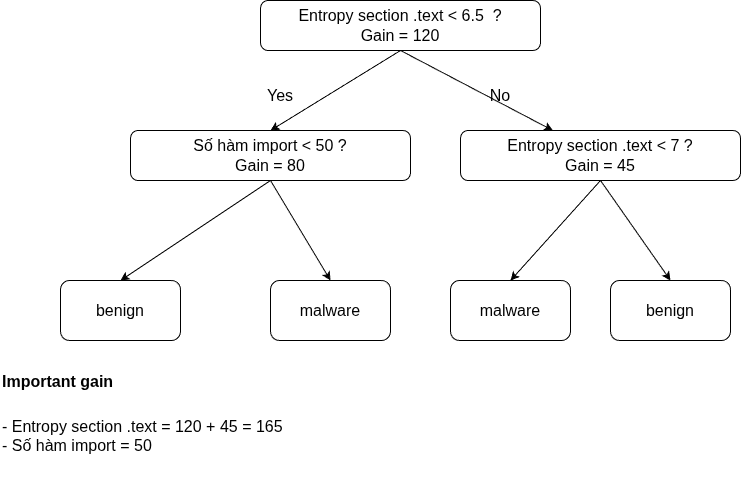
\includegraphics[width=\linewidth]{Hinhve/Pic3gain.png}
  \caption{Minh họa cách tính Importance Gain.}
  \label{fig:importance_gain}
\end{figure}
Phương pháp này có ưu điểm là được tính sẵn trong quá trình huấn 
luyện mà không cần bước đánh giá riêng. Sau khi huấn luyện, các đặc 
trưng được xếp hạng theo Gain giảm dần và chỉ giữ lại top--K đặc 
trưng có giá trị cao nhất để huấn luyện lại mô hình với số chiều nhỏ 
hơn.

\section{Phân tích động và giám sát hành vi}
\label{section:2.4}

\subsection{Khái niệm sandbox và phân tích động}
\label{section:2.4.1}
Phân tích động thực thi tệp nghi ngờ trong một sandbox nhằm quan sát
trực tiếp hành vi của chương trình lúc chạy~\cite{gibert2020}. Các
hành vi thường được theo dõi gồm tạo, sửa đổi hoặc xóa tệp, thay đổi
khóa Registry, tạo tiến trình con, nạp thư viện động và thiết lập kết
nối mạng; trước mỗi lần phân tích, sandbox được khôi phục về trạng
thái ban đầu để bảo đảm tính độc lập giữa các lần chạy.

So với phân tích tĩnh, phân tích động quan sát được hành vi thực tế
ngay cả khi mẫu bị đóng gói hoặc mã hóa, nhưng tiêu tốn nhiều tài
nguyên và thời gian hơn và có thể bị né tránh bởi các kỹ thuật phát
hiện môi trường ảo hóa~\cite{gibert2020}.

\subsection{Sysmon}
\label{section:2.4.2}
Sysmon là công cụ giám sát hệ thống thuộc bộ
Sysinternals của Microsoft, ghi lại các hoạt động chi tiết trên
Windows~\cite{sysmon}. Về kiến trúc, Sysmon gồm một driver kernel-mode
đăng ký callback để ghi nhận sự kiện hệ thống ở mức thấp, và một dịch
vụ user-mode chuẩn hóa dữ liệu rồi ghi vào Windows Event
Log~\cite{sysmon}. Hình~\ref{fig:sysmon_architecture} minh họa kiến
trúc hai tầng này.
\begin{figure}[H]
  \centering
  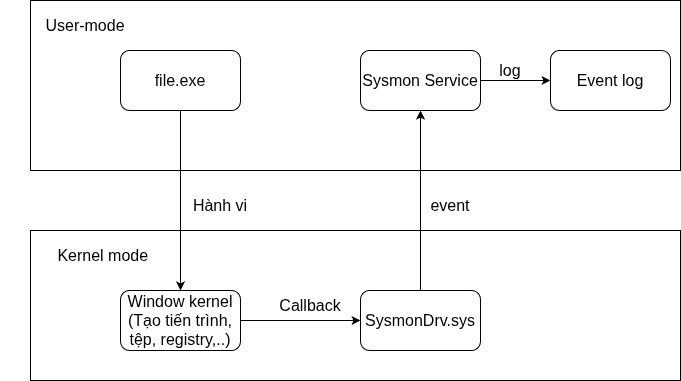
\includegraphics[width=\linewidth]{Hinhve/Pic4Sysmon.png}
  \caption{Minh họa kiến trúc Sysmon.}
  \label{fig:sysmon_architecture}
\end{figure}
Phần lớn mã độc chạy ở user-mode (tầng đặc quyền thấp dành cho ứng dụng
thông thường), nhưng mọi thao tác tạo tiến trình, ghi tệp, sửa registry
hay kết nối mạng của chúng đều phải đi qua kernel để được thực thi. Nhờ
đặt cảm biến tại driver kernel-mode --- tầng đặc quyền cao hơn nơi mã
độc user-mode hoạt động --- Sysmon ghi nhận được đầy đủ các hoạt động
này và khó bị mã độc vô hiệu hóa, khác với các công cụ giám sát chạy ở
user-mode vốn cùng tầng quyền với mã độc nên có thể bị qua mặt.

Một điểm mạnh của Sysmon là lượng thông tin đi kèm mỗi sự kiện. Ngoài
loại hành vi, một sự kiện Sysmon còn ghi nhiều trường ngữ cảnh như
đường dẫn và giá trị băm của tệp thực thi, dòng lệnh khởi chạy, cùng
tiến trình cha sinh ra nó. Nhờ các trường này, mỗi sự kiện mô tả hành
vi đầy đủ hơn so với nhật ký mặc định của Windows: quan hệ cha--con
giữa các tiến trình là cơ sở để tái dựng cây tiến trình, còn đường dẫn,
dòng lệnh và giá trị băm là nguồn để rút ra các chỉ số xâm phạm.

Mỗi loại sự kiện được Sysmon ghi lại với một mã định danh riêng gọi là
Event ID. Sysmon cho phép cấu hình linh hoạt thông qua tệp XML, trong
đó người dùng xác định loại sự kiện cần thu thập và điều kiện lọc tương
ứng để tập trung vào các hành vi đáng ngờ và giảm lượng dữ liệu nhiễu
từ các tiến trình hệ thống thông thường~\cite{sysmon}. Bảng~\ref{tab:sysmon_eid}
liệt kê các EID được sử dụng trong đồ án này.
\begin{table}[H]
\centering
\caption{Các Event ID của Sysmon được sử dụng trong đồ án.}
\label{tab:sysmon_eid}
\begin{tabular}{|c|l|p{9cm}|}
\hline
\multicolumn{1}{|c|}{\textbf{EID}} & \multicolumn{1}{c|}{\textbf{Sự kiện}} & \multicolumn{1}{c|}{\textbf{Ý nghĩa}} \\
\hline
1  & Process Create        & Ghi nhận tiến trình mới được tạo \\
\hline
2  & File Creation Time    & Thay đổi timestamp của tệp (ngụy trang) \\
\hline
3  & Network Connection    & Kết nối mạng được thiết lập từ tiến trình \\
\hline
5  & Process Terminate     & Tiến trình kết thúc \\
\hline
6  & Driver Load           & Trình điều khiển (driver) được nạp \\
\hline
7  & Image Load            & DLL được nạp vào tiến trình \\
\hline
8  & CreateRemoteThread    & Tạo luồng trong tiến trình khác (dấu hiệu tiêm mã) \\
\hline
9  & Raw Disk Access       & Truy cập trực tiếp ổ đĩa \\
\hline
10 & Process Access        & Truy cập bộ nhớ tiến trình khác \\
\hline
11 & File Create           & Tệp mới được tạo \\
\hline
12 & Registry Event        & Tạo hoặc xóa khóa registry \\
\hline
13 & Registry Value Set    & Giá trị registry được thay đổi \\
\hline
14 & Registry Key Rename    & Đổi tên khóa/giá trị registry \\
\hline
15 & FileCreateStreamHash   & Ghi dữ liệu vào Alternate Data Stream (ADS) \\
\hline
17 & Pipe Created          & Named pipe được tạo \\
\hline
18 & Pipe Connected        & Kết nối vào named pipe \\
\hline
19 & WMI Event Filter      & Đăng ký WMI event filter \\
\hline
20 & WMI Event Consumer    & Tạo WMI consumer \\
\hline
21 & WMI Event Binding     & Liên kết WMI filter và consumer \\
\hline
22 & DNS Query             & Truy vấn DNS \\
\hline
23 & File Delete           & Tệp bị xóa \\
\hline
25 & Process Tampering     & Phát hiện chỉnh sửa bất thường tiến trình \\
\hline
26 & File Delete Logged    & Ghi nhận sự kiện xóa tệp \\
\hline
\end{tabular}
\end{table}
\subsection{ETW và SilkETW}
\label{section:2.4.3}

Sysmon chủ yếu thu thập sự kiện ở mức hệ điều hành; cơ chế này không
phản ánh các hoạt động bên trong .NET Runtime. Ngày càng nhiều mã độc
Windows được viết bằng .NET và thực thi theo kiểu fileless, nạp payload
thẳng vào bộ nhớ để né phân tích tĩnh~\cite{elastic_dotnet}. Hai kỹ
thuật tiêu biểu là nạp assembly từ bộ nhớ bằng
\texttt{Assembly.Load} (không ghi tệp ra ổ đĩa) và sinh mã động bằng
\texttt{Reflection.Emit} (tự sinh mã thực thi ngay lúc chạy); cả hai
không tạo tệp trên đĩa nên Sysmon không quan sát được.

ETW là cơ chế ghi nhận sự kiện tích hợp
sẵn trong Windows theo mô hình provider~\cite{microsoft_etw}. .NET
Runtime được Microsoft trang bị sẵn provider \texttt{DotNETRuntime}:
mỗi khi Runtime nạp assembly hoặc gọi phương thức, provider tự động
phát sự kiện tương ứng --- cơ chế này nằm ngoài tầm kiểm soát của mã
độc. SilkETW là công cụ mã nguồn mở do FuzzySecurity phát triển, đăng
ký lắng nghe ETW provider và xuất sự kiện ra tệp JSON~\cite{silketw}.
Hình~\ref{fig:sysmon_etw} so sánh hai nguồn sự kiện: Sysmon nhận
callback từ kernel khi chương trình gọi API hệ điều hành, còn ETW nhận
sự kiện do .NET Runtime tự phát ra từ bên trong.
\begin{figure}[H]
\centering
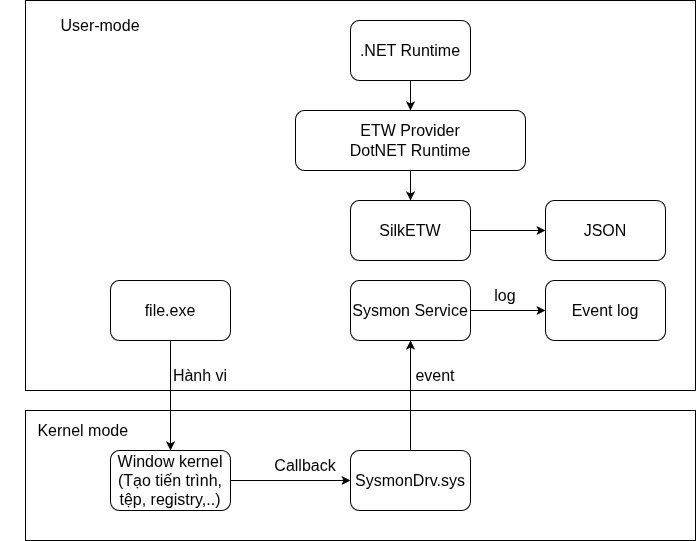
\includegraphics[width=\linewidth]{Hinhve/Pic5Sysmon_ETW.png}
\caption{So sánh phạm vi giám sát của Sysmon và ETW.}
\label{fig:sysmon_etw}
\end{figure}
Provider \texttt{DotNETRuntime} phát sự kiện cho tất cả chương trình
.NET đang chạy, không chỉ mẫu đang phân tích; dữ liệu thu được cần
lọc theo PID của mẫu trước khi xử lý, như trình bày tại
Chương~\ref{chapter:Implementation}.

\subsection{Chuỗi hành vi và chỉ số xâm phạm}
\label{section:2.4.4}

Các sự kiện đơn lẻ thu được từ Sysmon và ETW thường chưa đủ để đánh
giá mức độ nguy hiểm của một mẫu, do nhiều hành vi tương tự cũng có
thể xuất hiện trong phần mềm hợp pháp. Các sự kiện do đó cần được
tổng hợp thành biểu diễn có cấu trúc ở mức cao hơn nhằm mô tả toàn
bộ hành vi của mẫu.

Chuỗi hành vi là tập hợp các sự kiện được
sắp xếp theo thứ tự thời gian và có thể được nhóm theo loại
hành vi. Cách biểu diễn này cho phép quan sát luồng thực thi
tổng thể của mẫu thay vì các sự kiện rời rạc. Ví dụ, một mẫu
có thể lần lượt thực hiện tạo tiến trình con, ghi tệp thực
thi, thiết lập kết nối mạng và cấu hình cơ chế tự khởi động,
qua đó phản ánh chuỗi hành vi ở mức chiến thuật.

IOC là các dấu hiệu
cụ thể trích xuất từ hành vi của mẫu, dùng để nhận diện hoặc truy vết
mã độc trên các hệ thống khác. IOC bao gồm địa chỉ IP, tên miền, URL,
đường dẫn tệp được tạo hoặc chỉnh sửa, giá trị băm, khóa
registry bị thay đổi và tên named pipe. IOC hỗ trợ điều tra sự cố
bằng cách cho phép đối chiếu nhanh giữa các hệ thống để phát hiện dấu
hiệu lây nhiễm tương tự.

\subsection{Khung MITRE ATT\&CK}
\label{section:2.4.5}

MITRE ATT\&CK
là cơ sở tri thức mở do MITRE phát triển, mô tả và phân loại các kỹ
thuật tấn công mạng dựa trên quan sát thực tế từ các sự cố an ninh
toàn cầu~\cite{mitre_attack}.

Khung ATT\&CK được tổ chức theo cấu trúc phân cấp gồm ba mức. Cấp 
cao nhất là chiến thuật (Tactic), mô tả mục tiêu của kẻ tấn công 
trong từng giai đoạn, ví dụ như duy trì quyền truy cập (Persistence) 
hoặc thu thập dữ liệu (Collection). Cấp tiếp theo là kỹ thuật (Technique), mô tả cách thức cụ thể để đạt
được mục tiêu đó — ví dụ: tạo khóa registry Run để tự khởi động
(T1547.001) hoặc tiêm mã vào tiến trình khác (T1055). Cấp cuối cùng là kỹ thuật con (Sub-technique), cung cấp 
mức độ chi tiết hơn của từng kỹ thuật cụ thể.

Trong phân tích mã độc, việc ánh xạ các hành vi quan sát được sang 
các kỹ thuật trong MITRE ATT\&CK giúp chuẩn hóa mô tả hành vi, đồng 
thời hỗ trợ việc suy luận ngữ cảnh tấn công ở mức cao hơn thay vì chỉ 
dựa trên các sự kiện rời rạc~\cite{mitre_attack}.

\section{Các công trình liên quan}
\label{section:2.5}

Cuckoo Sandbox và Any.Run là các hệ thống phân tích động được sử dụng
rộng rãi, thu thập hành vi mẫu qua lời gọi API, lưu lượng mạng và
thay đổi hệ thống tệp, tổng hợp thành báo cáo IOC cho nhà phân
tích~\cite{gibert2020}. Hai hệ thống này chủ yếu dựa vào kỹ thuật can
thiệp lời gọi API ở user-mode, vốn có thể bị mã độc phát
hiện và vô hiệu hóa, đồng thời chưa quan sát sâu hoạt động thực thi
trong .NET Runtime. Về hướng học máy trên đặc trưng tĩnh PE, Anderson
và Roth đề xuất bộ đặc trưng EMBER và mô hình LightGBM với hiệu quả
cao trên dữ liệu quy mô lớn~\cite{ember2018}; Choudhary et al. mở rộng
hướng này bằng lựa chọn đặc trưng, giảm số chiều từ 2.381 xuống 384
trên các tập EMBER, BODMAS và ERMDS~\cite{choudhary2025}. Tuy nhiên,
các phương pháp tĩnh thuần túy mất tính phân biệt khi tệp PE bị đóng
gói, do cấu trúc quan sát được khác xa tệp gốc.

Đồ án kế thừa bộ đặc trưng EMBER và đánh giá ba thuật toán phân loại
trên tập dữ liệu tự thu thập, đồng thời tích hợp phân tích động với
Sysmon và SilkETW để thu thập chuỗi hành vi, IOC và ánh xạ MITRE
ATT\&CK. Khác với Cuckoo và Any.Run, đồ án khai thác trực tiếp ETW
provider của .NET Runtime thay vì can thiệp lời gọi API, nhờ đó quan
sát được các kỹ thuật thực thi trong bộ nhớ mà phân tích tĩnh và Sysmon
khó ghi nhận, đồng thời giảm khả năng bị mã độc phát hiện môi trường
phân tích. Việc bổ sung giai đoạn động cũng giúp xử lý các mẫu bị đóng
gói — tình huống mà đặc trưng tĩnh kém hiệu quả.

Những khác biệt trên được tổng hợp trong Bảng~\ref{tab:related-comparison},
đặt đồ án bên cạnh hai hệ thống phân tích động phổ biến để làm rõ vị trí
của hướng tiếp cận. Điểm phân biệt rõ nhất là cơ chế thu thập: trong khi
Cuckoo và Any.Run can thiệp lời gọi API ở user-mode, đồ án quan sát ở mức
kernel qua Sysmon kết hợp ETW của .NET Runtime, nhờ đó vừa khó bị mã độc
phát hiện, vừa nhìn được hoạt động thực thi trong bộ nhớ mà hai hệ thống
kia khó ghi nhận.
\begin{table}[H]
\centering
\setlength{\tabcolsep}{4pt}
\caption{So sánh đặc điểm giữa đồ án và các hệ thống phân tích động
  hiện có~\cite{gibert2020}.}
\label{tab:related-comparison}
\begin{tabular}{|p{4.6cm}|c|c|c|}
\hline
\multicolumn{1}{|c|}{\textbf{Đặc điểm}} & \multicolumn{1}{c|}{\textbf{Cuckoo}} & \multicolumn{1}{c|}{\textbf{Any.Run}} & \multicolumn{1}{c|}{\textbf{Đồ án}} \\
\hline
Cơ chế thu thập động & API hooking & API hooking & Sysmon + ETW \\
\hline
Quan sát .NET trong bộ nhớ & Hạn chế & Hạn chế & Có \\
\hline
Kháng phát hiện hook & Thấp & Trung bình & Cao \\
\hline
Phân loại tĩnh bằng học máy & Không & Không & Có \\
\hline
Hợp nhất tĩnh--động & Không & Không & Có \\
\hline
Ánh xạ MITRE ATT\&CK & Một phần & Có & Có \\
\hline
Mã nguồn mở / tự triển khai & Có & Không & Có \\
\hline
\end{tabular}
\end{table}
Các cơ sở trên cho thấy phân tích tĩnh và phân tích động bù trừ cho
nhau: đặc trưng tĩnh PE cho phép phân loại nhanh nhưng mất tác dụng khi
mẫu bị đóng gói, còn giám sát động bằng Sysmon kết hợp ETW quan sát
được hành vi thực --- kể cả hoạt động .NET trong bộ nhớ mà Sysmon bỏ
sót. Đây là căn cứ để đồ án kết hợp hai hướng trong thiết kế ở
Chương~\ref{chapter:Design}.

\end{document}